\documentclass{article}

\usepackage{pdfpages}
\usepackage{graphicx}
\usepackage{longtable}
%\usepackage[export]{adjustbox}
%\usepackage{tabu}
\usepackage{xcolor,colortbl}
\usepackage{caption}
\usepackage{subcaption}
\usepackage{float}
\usepackage{wrapfig}
\usepackage[margin=0.65in]{geometry}
\usepackage{url} % for bibliograpy links
\begin{document}

\vspace*{3ex}
\begin{flushright}
{\large 10 November 2015}
\end{flushright}

\vskip20ex
\hskip3cm

\begin{center}


\begin{figure}[H]
\centering
\begin{subfigure}{.5\textwidth}
  \centering
  
\includegraphics[width=.9\linewidth]{images/mini.png}
\end{subfigure}%
\begin{subfigure}{.5\textwidth}
  \centering
  
\includegraphics[width=.9\linewidth]{images/pw.jpg}
\end{subfigure}
\end{figure}




\Large {\bf
	Bachelor Thesis \\
	Finite Automata for Pattern Recognition
}

\Large {\bf 
	Technical Project
}
\end{center}
\vskip2ex


\vskip25ex

\begin{flushleft}
{\large Bartlomiej Dybisz \\
Jakub Ciecierski

}
\end{flushleft}

\newpage
\tableofcontents
\newpage

%------------------------------------------------------------------------------

\section*{Document metric}

\begin{center}


\begin{table}[h]
\hspace*{-1.1cm}
\large
\begin{tabular}{|
>{\columncolor[HTML]{C0C0C0}}l |l|l|l|l|l|}
\hline
\multicolumn{6}{|l|}{\cellcolor[HTML]{C0C0C0}Document metric}                                                                                                                                         \\ \hline
Project:       & \multicolumn{2}{l|}{Finite automata for pattern recognition} & 
\cellcolor[HTML]{C0C0C0}Company: & \multicolumn{2}{l|}{WUT}                                               \\ \hline
Name:          & \multicolumn{5}{l|}{Technical Project}                                                                                                                                       \\ \hline
Topics:        & \multicolumn{5}{l|}{Architecture and algorithms defining the project}                                                                                                                                       \\ \hline
Author:        & \multicolumn{5}{l|}{Jakub Ciecierski, Bartlomiej Dybisz}                                                                                                                                                \\ \hline
File:          & \multicolumn{5}{l|}{technical\_project.pdf}                                                                                                                                      \\ \hline
Version no:    & 0.1                                                                      & \cellcolor[HTML]{C0C0C0}Status:  & Under development & \cellcolor[HTML]{C0C0C0}Opening date: & 2015-10-27 \\ \hline
Summary:       & \multicolumn{5}{l|}{Technical side of research on pattern recognition by finite automata}                                                                                                           \\ \hline
Authorized by: & \begin{tabular}[c]{@{}l@{}}Wladyslaw Homenda\end{tabular} & \multicolumn{3}{l|}{\cellcolor[HTML]{C0C0C0}Last modification date:}                         & 2015-11-10 \\ \hline
\end{tabular}
\end{table}

\end{center}



\section*{History of changes}

\begin{center}


\begin{table}[h]
\hspace*{-1.0cm}
\large
\begin{tabular}{|l|l|l|l|}
\hline
\multicolumn{4}{|l|}{\cellcolor[HTML]{C0C0C0}History of Changes} \\ \hline
Version         & Date         & Who        & Description        \\ \hline

0.1         
& 2015-11-10
& Jakub Ciecierski, Bartlomiej Dybisz
& Definition of the main purpose of the document       \\ \hline
\end{tabular}
\end{table}

\end{center}


%---------------------------------------------------------------

\section*{Schedule}

\begin{center}


\begin{table}[h]

\large
\begin{tabular}{|l|l|l|}
\hline
\multicolumn{3}{|l|}{\cellcolor[HTML]{C0C0C0}Schedule} \\ \hline
Date         & Note        & Planned Progress          \\ \hline
\hline

27.10.2015   & Lab1    & Presentation of Business Analysis   \\ \hline
03.11.2015   &    & Additional changes of Business Analysis   \\ \hline
7-9.11.2015   &     & First drafts of UML of particular modules   \\ \hline
14-16.11.2015   &     & Requirements analysis, design of algorithms and further UML development \\ \hline
17.11.2015   &  Lab2   & Presentation of Technical Analysis   \\ \hline
20-22.11.2015   &     & Implementation of mudules needed for testing and basic GUI   \\ \hline
31.11.2015   & Lab3    & Presentation of results of tests on synthetic and semi-synthetic data  \\ \hline
4-6.12.2015   &     & GUI and console application development  \\ \hline
15.12.2015   & Lab4    & Final GUI  \\ \hline
-------  & -------    & Work depends on acquired results  \\ \hline
08.01.2015  & Lab5    & Complete system presentation  \\ \hline
\end{tabular}
\end{table}

\end{center}


%---------------------------------------------------------------
\newpage




%---------------------------------------------------------------
\section{Production Model}
{\bf Waterfall} model is a model which was developed for software development; that is to create software. It is called as such because the model develops systematically from one phase to other in a downward fashion, like a waterfall.

{\color{red} NICE DECRIPTION LOL2}

\begin{center}

	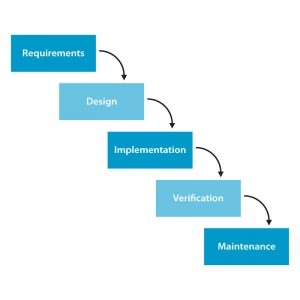
\includegraphics[width=80mm]{images/waterfall_model.jpg}

\end{center}


%---------------------------------------------------------------
\section{Technology}

%---- JC ----%


%---- BD ----%
\subsection{Graphical User Interface}

%LOL
\begin{wrapfigure}{c}{0.5\textwidth}
  \begin{center}
    
\includegraphics[width=0.3\textwidth]{images/javafx_logo.png}
  \end{center}
\end{wrapfigure}

To create Graphical User Interface, we will use JavaFx technology. It is a set of graphics and media packages that enables developers to design, create, test, debug, and deploy rich client applications that operate consistently across diverse platforms. Written as a Java API, JavaFX application code can reference APIs from any Java library. For example, JavaFX applications can use Java API libraries to access native system capabilities and connect to server-based middleware applications \cite{javafx_description}. Since GUI will be simple and straight forward, this technology will provide cross-platform character of the application and help us develop it in no time. Only basic user interface elements such as buttons, text fields, label etc will be used, hence we do not demand any sophisticated API.




\newpage


%---------------------------------------------------------------
\section{Algorithms} \label{section:Algorithms}

%---- JC ----%


%---- BD ----%


%---------------------------------------------------------------
%---------------------------------------------------------------
\subsubsection{Examples}
% Examples of algorithms, if any.

%---- JC ----%


%---- BD ----%

%---------------------------------------------------------------
\section{Data structures}

%---- JC ----%


%---- BD ----%

%---------------------------------------------------------------
\section{Modules}
	
%---- JC ----%


%---- BD ----%

%---------------------------------------------------------------
\section{Modelling}
\textcolor{red}{Remark:} What should be stress out is that class diagrams presented in this section may not cover all methods needed to implement full functionality. For sure presented methods are neccessary, but not always sufficient. Although we were trying to be as precise as we can, they constitutes only a sketch of solution.


%---- JC ----%


%---- BD ----%

%
% WORD PROCESSING CLASS DIAGRAM
%
\newpage
\subsection{Words Processing}
To perform words generation/processing we will use classes presented on figure \ref{fig:words_processing_class}.

Since it happens to be largest and most important of all four, let us first focus on \texttt{WordsGenerator} class. Its main purpose is to create words using rules described in section \ref{section:Algorithms}. There are in fact two type of conditions to cover:
\begin{itemize}
\item parametrical, where the class checks global parameters related to word processing
\item hamming condition, generated word of some length, let us say $n$, must have hamming distance between all (up to now) generated words of length $n$ smaller than some defined constant (see \ref{section:Algorithms} for reference)
\end{itemize}

Check of the first one is done via \texttt{\_checkGlobalConsitions()} and latter one is covered by \texttt{\_hammingCondition()}. As one can easily see, \texttt{\_hammingDistance()} method is just an auxiliary procedure for work related to checking hamming condition. Although method \texttt{\_generateRandomWordOverAlphabet} speaks for itself, \texttt{\_generateRandomWordStartinWith} needs some explanation. As we are forced to firstly produce words starting with different symbols of alphabet (again section \ref{section:Algorithms}), this method provides a way to create such a word with hamming condition checked. User specifies only starting symbol and length of the word and procedure returns random word starting with particular symbol and of specified length. There are only two public methods: constructor, which forces user to specify alphabet and \texttt{getPairs()}. The last one's ability is to gather all generated words and combine them into pairs. Such approach is forced by PSO's fitness function. 

Despites its vague name, \texttt{BagOfWords} is class which preserves set of words in form of an unordered map, where keys are lengths and entries are vectors of words of specified length. It enables easy access to words of some particular length. We took such approach because most comparisions in the \texttt{WordsGenerator} class is done by checking hamming condition, which concerns words of the same length. What is more, section \ref{section:Algorithms} obliged us to create 3 disjunctive sets of words: $\Omega_S$, $\Omega_M$ and $\Omega_L$ and using this class we can fulfil this need, preserving all desired functionality. When needed one can always gather all words as a vector using \texttt{getAllWords()} method.

Last two classes were created to make code more transparent. \texttt{PairOfWords} simply wraps two words together and \texttt{Word} class supplies user with short set of methods operating on vector of integers (which simulates a word). As mentioned they are more needed because their names than actual functionalites.

\begin{figure}[H]
	\centering
	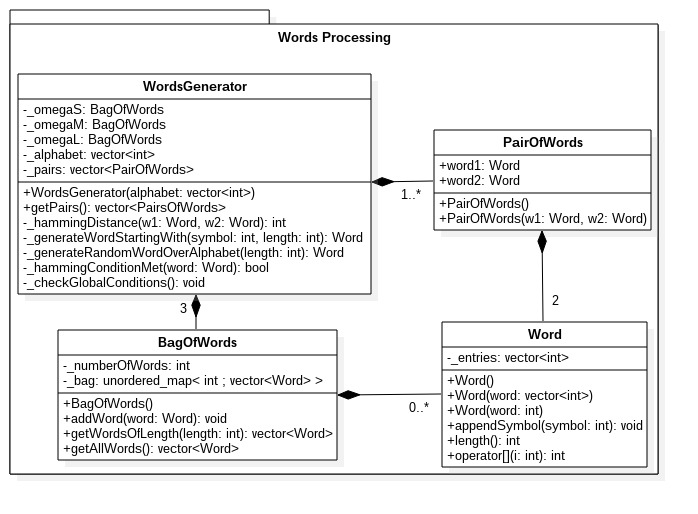
\includegraphics[width=0.8\textwidth]{images/words_processing.jpg}
    \caption{Class diagram of words processing clases.}
    \label{fig:words_processing_class}
\end{figure}

%
% TRANSITION TABLE CLASS DIAGRAM
%
\newpage
\subsection{Transition Table}
Classes used to model behaviour of transition table are presented on figure \ref{fig:trans_table_class}. 

\textcolor{red}{Remark:} It is worth to notice that in all consecutive classes, entries of transition tables stays as a vector of integers. Each table, beginning with \texttt{StandardTransitionTable}, provides its own way to read values from the vector either via overloading \texttt{operator ()} or by implementing methods.

As one can see, starting from most general \texttt{TransitionTable} and going up on chains of inheritance classes broad they abilities. Base class provides only methods for loading automaton from file specified via \texttt{url} string. It is able to either load it symbol by symbol ( \texttt{\_loadOneSymbol()} ) or fill up all entries at once - \texttt{\_loadEntries()}. Entries at this level can not be interpreted using any transition table type - it is just raw data.

Next, one can create \texttt{StandardTransitionTable}, which interprets \texttt{\_entries} as a table where columns represents symbols and rows are states. Classes, which will inherit from this one are provided with method \texttt{\_accessTransitionTable()} and for public usage \texttt{operator ()} has been overloaded. Both approaches force to pass symbol and state and as a results guarantee state. 

Thrid  is \texttt{PerSymbolTransitionTable}, which is more suited for computer interpretation of automaton. It assumes that each symbol has its own table. Each table's column and rows represents consecutive states and entries takes values equal to either $0$ or $1$. Such a values describe situation when "two states are not connected" and "there is connection between states", repsectively. Simmiraly to \texttt{StandardTransitionTable}, there are two ways to acces table. Public access is provided by overloaded \texttt{operator ()} and protected access is anabled via \texttt{\_isTransition()} method. Both needs two states and symbol to determine whether there is connection or not, hence return value is of boolean type.

Last but not least, we have \texttt{CodedTransitionTable} class. First observable difference appears in constructors - this class enables to initialize transition table either via loading and coding automaton from file or accepting coded automaton and decoding it to achieve transition table. Such approach has been forced by Particle Swarm Optimization algorithm. TO be a little bit more precise: paticles are represented by coded deterministic finite automata and need to be updated, which causes automata to change. In such a case we just create new automaton from updated particle's coded DFA table. \texttt{\_getCodedTransitionTable}, as name says, returns coded table, which then can be used as a position of particle within PSO space. All other methods concerns either coding or decoding procedures and are described more in section \ref{section:Algorithms}.




\begin{figure}[H]
	\centering
	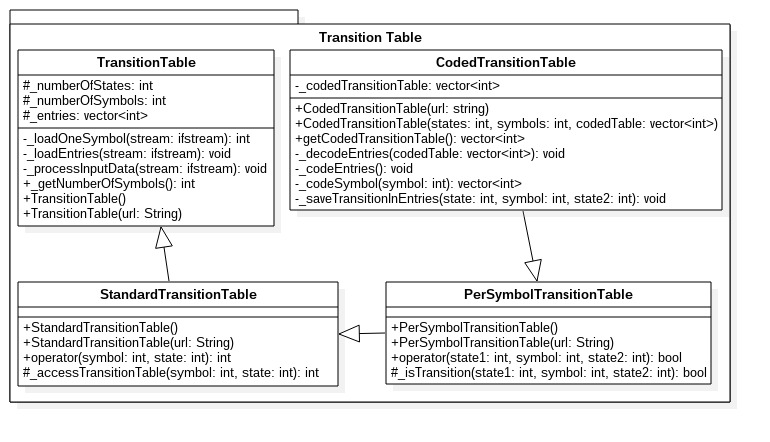
\includegraphics[width=0.9\textwidth]{images/transition_table.jpg}
    \caption{Class diagram of classes implementing different transition tables notations.}
    \label{fig:trans_table_class}
\end{figure}


\section{Bibliography}

\begin{thebibliography}{1}
	\bibitem{javafx_description} \url{http://docs.oracle.com/javafx/2/overview/jfxpub-overview.htm}	
\end{thebibliography}



\end{document}


